\documentclass[11pt]{amsbook}

\makeatletter
\def\@thm#1#2#3{%
  \ifhmode\unskip\unskip\par\fi
  \normalfont
  \trivlist
  \let\thmheadnl\relax
  \let\thm@swap\@gobble
  \let\thm@indent\indent % indent
  \thm@headfont{\bfseries}% heading font boldface // changed
  \thm@notefont{\fontseries\mddefault\upshape}%
  \thm@headpunct{.}% add period after heading
  \thm@headsep 5\p@ plus\p@ minus\p@\relax
  \thm@space@setup
  #1% style overrides
  \@topsep \thm@preskip               % used by thm head
  \@topsepadd \thm@postskip           % used by \@endparenv
  \def\@tempa{#2}\ifx\@empty\@tempa
    \def\@tempa{\@oparg{\@begintheorem{#3}{}}[]}%
  \else
    \refstepcounter{#2}%
    \def\@tempa{\@oparg{\@begintheorem{#3}{\csname the#2\endcsname}}[]}%
  \fi
  \@tempa
}
\makeatother

\renewcommand{\chaptername}{Lecture}

\usepackage[T1]{fontenc}
\usepackage[latin1]{inputenc}
\usepackage{times}
\usepackage{microtype}
\usepackage{amssymb}
\usepackage{a4wide}
\usepackage{graphicx}
%\usepackage{paralist}
%\usepackage{bbm}
\usepackage[pagebackref]{hyperref} 
\hypersetup{pdftitle={\title}, pdfauthor={\author}}
\usepackage{verbatim}
\usepackage{url}
\usepackage[pagebackref]{hyperref}
\hypersetup{pdftitle={\title}, pdfauthor={\author}}

\newcommand{\ba}{{\boldsymbol{a}}}
\newcommand{\balpha}{{\boldsymbol{\alpha}}}
\newcommand{\bb}{{\boldsymbol{b}}}
\newcommand{\bc}{{\boldsymbol{c}}}
\newcommand{\be}{{\boldsymbol{e}}}
\newcommand{\bff}{{\boldsymbol{f}}}
\newcommand{\bnu}{{\boldsymbol{\nu}}}
\newcommand{\bm}{{\boldsymbol{m}}}
\newcommand{\bo}{{\boldsymbol{0}}}
\newcommand{\bp}{{\boldsymbol{p}}}
\newcommand{\bq}{{\boldsymbol{q}}}
\newcommand{\br}{{\boldsymbol{r}}}
\newcommand{\bsigma}{{\boldsymbol{\sigma}}}
\newcommand{\bt}{{\boldsymbol{t}}}
\newcommand{\bv}{{\boldsymbol{v}}}
\newcommand{\bw}{{\boldsymbol{w}}}
\newcommand{\bx}{{\boldsymbol{x}}}
\newcommand{\by}{{\boldsymbol{y}}}
\newcommand{\bz}{{\boldsymbol{z}}}
\newcommand{\bone}{{\boldsymbol{1}}}

\newcommand{\RR}{\mathbb{R}}
\newcommand{\Rgeo}{{\mathbb{R}_{\ge0}}}
\newcommand{\Zgeo}{{\mathbb{Z}_{\ge0}}}
\newcommand{\NN}{\mathbb{N}}
\newcommand{\ZZ}{\mathbb{Z}}
\newcommand{\QQ}{\mathbb{Q}}
\newcommand{\CC}{\mathbb{C}}

\newcommand{\cA}{{\mathcal{A}}}
\newcommand{\cC}{{\mathcal{C}}}
\newcommand{\cD}{{\mathcal{D}}}
\newcommand{\cH}{{\mathcal{H}}}
\newcommand{\cL}{{\mathcal{L}}}
\newcommand{\cO}{{\mathcal{O}}}
\newcommand{\cP}{{\mathcal{P}}}

\newcommand{\scp}[2]{\langle #1,#2\rangle}
\newcommand{\fl}[1]{\left\lfloor #1\right\rfloor}
\newcommand{\ce}[1]{\left\lceil #1\right\rceil}
\newcommand{\rcone}[1]{{{}_\Rgeo\!\left\langle #1\right\rangle}}
\newcommand{\zcone}[1]{{{}_\Zgeo\!\left\langle #1\right\rangle}}

\DeclareMathOperator{\interior}{int}
\DeclareMathOperator{\relint}{relint}
\DeclareMathOperator{\conv}{conv}
\DeclareMathOperator{\cone}{cone}
\DeclareMathOperator{\aff}{aff}
\DeclareMathOperator{\vol}{vol}
\DeclareMathOperator{\dist}{dist}
\DeclareMathOperator{\vertices}{vert}
\DeclareMathOperator{\rang}{rang}
\DeclareMathOperator{\sign}{sign}
\DeclareMathOperator{\pyr}{pyr}
\DeclareMathOperator{\bipyr}{bipyr}
\DeclareMathOperator{\Sl}{Sl}
\DeclareMathOperator{\im}{Im}
\DeclareMathOperator{\colspan}{colspan}
\DeclareMathOperator{\rank}{rank}

\DeclareMathOperator{\sgn}{sgn} %signum
\DeclareMathOperator{\ggT}{ggT}

\newcommand{\ojo}[1]{\textsf{\bfseries\boldmath #1}}
\newcommand{\scribe}[1]{\begin{center}\emph{Scribe: #1}\end{center}\bigskip}

\graphicspath{{graphics/}}

\numberwithin{equation}{section}

\newtheorem{theorem}{\textbf{Theorem}}[section]
\newtheorem{lemma}[theorem]{Lemma}
\newtheorem{proposition}[theorem]{Proposition}
\newtheorem{corollary}[theorem]{Corollary}
\newtheorem{conj}[theorem]{Conjecture}
\newtheorem{obs}[theorem]{Observation}
\newtheorem{exercise}[theorem]{Exercise}
\newtheorem{example}[theorem]{Example}
\newtheorem{remark}[theorem]{Remark}

\newtheorem{defn}{\textbf{Definition}}[section]

%\includeonly{lecture3}

\begin{document}

\thispagestyle{empty}

\newcommand{\thisyear}{2013}

\
\vfill
\begin{center}
        \Huge \sffamily\bfseries 
        Discrete and Algorithmic Geometry \thisyear
        \medskip
        (Part 2)

\vspace{2cm}
\LARGE
Julian Pfeifle

\vspace{3cm}

\normalfont\LARGE\sffamily
Version of \today

\vspace{5cm}\
\end{center}

This is the preliminary version of the lecture notes for the second
part of \emph{Discrete and Algorithmic Geometry} (Universitat
Polit�cnica de Catalunya), held in the fall semester of \thisyear\ by Ferran
Hurtado and Julian Pfeifle.

\medskip
These notes are fruit of the collaborative effort of all participating
students, who have taken turns in assembling this text. The name of
each scribe figures in each corresponding section.

\medskip
%The main literature for this course consists of
%\cite{Conway-Sloane-3rd}, \cite{Conway-Strauss08}
%and~\cite{Senechal95}. 

\medskip Suggestions for improvements will always be gladly received
by \texttt{julian.pfeifle@upc.edu}.

\vfill\


% Local Variables: 
% mode: latex
% TeX-master: "dag-upc"
% End: 

\tableofcontents

\chapter{Title of the lecture}

\scribe{Your name here}


% Local Variables: 
% mode: latex
% TeX-master: "dag-upc"
% End: 

\chapter{Asymptotic f-vectors of families of polytopes}

\scribe{Cecilia Gir\'on}

In this section we are going to study the \textit{unimodality conjecture} which says that there exists an $l = P(L)\in\mathbb{N}$ such that $f_0\leq f_1 \leq \cdots\leq f_l \leq f_{l+1}\leq \cdots \leq f_{d-1}\leq f_d$. We woould like to know if it is true. 

First, we define the \textbf{$f$-vector} as the vector of the form $(f_0,f_{1},\cdots,f_{d-1})$ where $f_i$ is as defined before in (\ref{eq1}). We will say that it is a \textbf{flag $f$-vector} $(f_s)_s = [d]$ such that $f_s$ count the number of flags $F_{i_1} \subset F_{i_2} \subset \cdots \subset F_{i_k}$ where $s = \{i_1,i_2,\cdots, i_k \}$ and $\dim F_{i_k} = i_k$ \footnote{You can also read about $cd$-index}.

\bigskip
The unimodal conjecture described before is known to be false for simplical polytopes of dimension $d\geq 19$ and for non-simplicial polytopes of dimension $d \geq 8$. The following conjecture is not known to be false. 

\textbf{Restricted unimodal conjecture (Anders Bjorner)}: 
\begin{eqnarray*}
 f_0\leq f_1\leq \cdots \leq f_{\lfloor \frac{d-1}{4}}\rfloor\\
 f_{\lfloor \frac{3(d-1)}{4}\rfloor}\geq \cdots \geq f_{d-1}
\end{eqnarray*} 

Intuitively we are sure that there is no way this conjecture could be false, but there is not proof of this. We don't even know if $f_k\geq \frac{1}{10000}\min\{f_0,f_{d-1}\}$ is true.

\bigskip

\textbf{Exercises done during the lecture 11/11/2013. Each one includes one}


\section{Operations on polytopes}
\begin{itemize}
\item \textbf{Cartesian (direct) product} $P\times Q$.
\item \textbf{Direct sum} $P^d \oplus q^e \subset \mathbb{R}^{d+e}$.
\item $P*Q\subset \mathbb{R}^{d+e+1}$. It is like $\oplus$ but the subspaces are skew (i.e. affine and they have no point on common). For example $\square^1 *\square^1 = Pyr(P)$.
\end{itemize}

\bigskip
\noindent\textsc{Example}: Given $f_k(P)$, calculate the $k$-th entry of $Pyr(P)$:
\begin{eqnarray*}
f(P)&=&(f_0,f_1,\cdots, f_{d-1}\\
f_k(Pyr(P)) &=& (f_0 +1, f_1 + f_0, f_2+f_1, \cdots, f_{d-2}+ f_{d-3}, f_{d-1}+ f_{d-2}, 1+ f_{d-1})
\end{eqnarray*}
\begin{flushright}
$\clubsuit$
\end{flushright}

\bigskip
\begin{itemize}
\item  \textbf{Connected sum} $P^d\#Q^d$ where $P$ has as simplicial face $f$ and $Q$ has a simplicial face $G$. 
\end{itemize}

This last operation is used to join the asymptotic function $f(\square^d)$ and its dual $f(\diamondsuit ^d)$. To make it work, since $\square^d$ has no triangulations in its faces, it is enough to cut away one vertex and, this way, get a simplex. Merging both functions using the connected sum gives place to a new function which is a non-unimodal function.


% Local Variables: 
% mode: latex
% TeX-master: "dag-upc"
% End: 

%\chapter{Pick's Theorem; Lattice packings of spheres}

\scribe{Miquel Ra\"{i}ch}

\section{Pick's Theorem}
\begin{theorem}[Pick]
Let $P$ be a lattice polygon in the plane ($P$ is closed, convex, simple and its vertices lie in $\ZZ^{2}$).
The area of $P$ is $$A(P)=\vol_{2}P=I+\frac{1}{2}B-1$$where:\\
$\mbox{    }\mbox{    } I=$ number of interior lattice points of $P$ $=\#\left\{(\mbox{int }P)\cap\ZZ^{2}\right\}$,\\
$\mbox{    }\mbox{    } B=$ number of boundary lattice points of $P$ $=\#\left\{\partial{}P\cap\ZZ^{2}\right\}$
\end{theorem}
\begin{proof}\mbox{[part]}\\
\begin{enumerate}
\item Show that Pick's formula is additive: if $P=P_1\cup{}P_2$, then $$I+\frac{1}{2}B-1=\left(I_1+\frac{1}{2}b_1-1\right)+\left(I_2+\frac{1}{2}B_2-1\right)$$
\begin{align*}A(P)=&A(P_1)+A(P_2)\\
I=I(P)=&I_1+I_2+L-2\\
B=B(P)=&B_1+B_2-2L+2\end{align*}
{\center (Principle of Inclusion-Exlusion $\rightarrow$ M\"obius function)\quad\quad\\[0.3cm]

\begin{minipage}{0.6\textwidth}$\lceil$ This proves:\begin{enumerate}\item Pick$(P_1\cup{}P_2)\Leftarrow$ Pick$(P_1)$, Pick$(P_2)$\\
\item Pick$(P_1)\Leftarrow$ Pick$(P_1\cup{}P_2)$, Pick$(P_2)$ $\rfloor$\end{enumerate}\end{minipage}}\\[0.5cm]

\item Prove it for lattice triangles.\end{enumerate}
\end{proof}

\section{Lattice packings of spheres}

A {\textbf{lattice-packing}} of congruent spheres ($\equiv$ same radius) in $\RR^{d}$ is a packing such that the set $Z=\{\mbox{centers of the spheres}\}$ is a lattice $L$ (free abelian group).

Let $\{v_1, \ldots, v_n\}\in\RR^{d}$ be a generating set for $$M=\left[\begin{array}{ccc}v_1 & \cdots & v_n\end{array}\right]\!\mbox{, then }L=\{M\lambda\colon\lambda\in\ZZ^{n}\}$$
$$M=\overbrace{\left.\left[\begin{array}{cc}1 & \frac{1}{2} \\ 0 & \frac{1}{2}\sqrt{3} \end{array}\!\right]\right\}}^{n}\!d\quad\quad\quad\quad\quad{}M\lambda=\left[\begin{array}{ccc}v_1 & \cdots & v_n\end{array}\right]\!\left[\begin{array}{c}\lambda_1 \\ \vdots \\ \lambda_n \end{array}\right]=\lambda_1{}v_1+\cdots+\lambda_n{}v_n$$\\[0.2cm]

Sphere packing $B_0+L=\{B_0+v\colon{}v\in{}L\}=\{B_0+M\lambda\colon\lambda\in\ZZ^{n}\}$
$$\forall{}p,q\in{}P,\mbox{ }\exists{}D_p, D_q\colon{}D_p\cap{}Dq=\emptyset\quad\quad\quad\quad{}p\in{}P\subset\RR^{d}\mbox{ discrete set of points}$$\\[0.1cm]
Voroni cell of $p$ w.r.t. $P$ is$$\mbox{Vor}(P)=\{y\in\RR^{d}\colon\lVert{}y-p\rVert\leq\lVert{}y-q\rVert\mbox{ }\forall{}q\in{}P\}$$
$\lceil$ Georges Voronoi (s. XIX) $\rfloor$\\[0.3cm]
Voronoi cells are intersections of half spaces$$\mbox{Vor}(P)=\bigcap_{q\in{}P}H_q\quad\quad\mbox{ where }H_q=\{y\in\RR^{d}\colon\lVert{}y-p\rVert\leq\lVert{}y-q\rVert\}$$

\begin{defn}\mbox{ }\\
$\mbox{    }\mbox{    } $polyhedron $\equiv^{def}$ intersection of half-spaces\\
$\mbox{    }\mbox{    } $polytope $\equiv^{def}$ convex hull of a finite point set $\overset{\text{FTPT}}{\equiv}$ bounded polyhedron\\[0.1cm]
{\small \upshape (FTPT: Fundamental theorem of polytope theory)}
\end{defn}\mbox{ }

\begin{enumerate}\item any convex hull of a finite point set is an intersection of half-spaces [easy by calculating convex hull].\\
\item any \underline{bounded} intersection of half-spaces is the convex hull of a finite set of points, unless the intersection is empty.\end{enumerate}\mbox{ }

Any lattice is isomorphic to some $\ZZ^n$, as abelian groups, by the map $v\in{}L\leftrightarrow\lambda\in\ZZ^n\colon{}v=M\lambda$

\mbox{ }\\[1.1cm]
[I will put images another day :P]

% Local Variables: 
% mode: latex
% TeX-master: "dag-upc"
% End: 
 
\chapter{The hexagonal lattice and laminated lattices}
\scribe{Ane Santos}

\section{The hexagonal lattice}

\begin{definition}
  Let $v_1,\ldots,v_n\in \ZZ^{d}$ and the lattice $L= {}_\ZZ\!\left\langle v_1,\ldots,v_n
  \right\rangle=\left\{\sum\lambda_i v_i : \lambda_i \in \ZZ\right\}=
  \left\{M\lambda:\lambda\in \ZZ^{n}\right\}$ with
  $M=\left[v_1,\ldots,v_n\right]\in\ZZ^{d\times n}$. $M$ is called the \emph{generator
    matrix} and ${}_\ZZ\!\left\langle v_1,\ldots,v_n \right\rangle$ the \emph{integer hull} of the
  lattice.
\end{definition}


We will study two variants of the hexagonal lattice:
\[
  A_{2,\RR^{2}}
  \ = \
  \left\{\begin{bmatrix}
        1 & 1/2 \\
        0 & \sqrt{3}/2 \end{bmatrix}\lambda:\lambda\in\ZZ^{2}\right\}, 
    \qquad
  A_{2,\RR^{3}}
  \ = \
  \left\{\begin{bmatrix}
        1 & 0 \\
        -1 & 1 \\
        0 & -1 \end{bmatrix}\lambda:\lambda\in\ZZ^{2}\right\},
\]
with respective generating matrices
$M=\left[\begin{smallmatrix}
      1 & 1/2 \\
      0 & \sqrt{3}/2 \end{smallmatrix}\right]$ and
$M'=\left[\begin{smallmatrix}
      1 & 0 \\
      -1 & 1 \\
      0 & -1 \end{smallmatrix}\right]$. 

Firstly, we study $A_{2,\RR^{3}}$:

\begin{figure}[htbp]
\centering
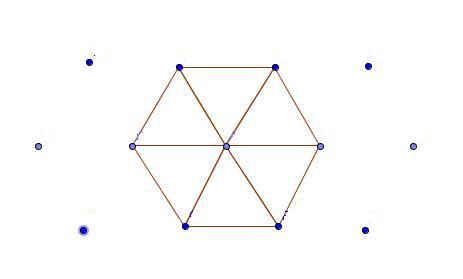
\includegraphics[width=0.5\textwidth]{apunteaklattice}
\caption{$A_{2,\RR^{3}}$}
\end{figure}


\begin{displaymath}
	A_{2,\RR^{3}}=\left\{M'\lambda:\lambda\in\ZZ^{2}\right\}=\left\{\begin{bmatrix}
	\lambda_1 \\
	-\lambda_1 + \lambda_2 \\
	-\lambda_2 \end{bmatrix}:\lambda_1,\lambda_2\in\ZZ\right\}
\end{displaymath}

We want to find a hyperplane that contains $A_{2,\RR^{3}}$. We are in $\RR^{3}$, so this
hyperplane is of the form $\left\{x\in\RR^{3}:\left\langle
    a,x\right\rangle=a_0\right\}$. But we know $0$ is in $A_{2,\RR^{3}}$ so $a_0=0$ and
\[
  H \ = \ 
  \left\{x\in\RR^{3}:\left\langle a,x\right\rangle=0\right\} 
  \ = \ 
  \left\{\omega\in\RR^{3}:\left\langle \omega,x\right\rangle, \forall \in \colspan
    M\right\},
\]
 where $\colspan
M={}_\RR\!\left\langle v_1,\ldots,v_n \right\rangle=\im M$ (it is an abelian group and it is
also a vector space). So, $H=\left\{x\in\RR^{3}: \left\langle
    a,x\right\rangle=0\right\}=\ker M$

$\dim \im M=2$ and $\dim A_{2,\RR^{3}}=3$ $\Longrightarrow$ $\dim A_{2,\RR^{3}}=\dim \ker M +\dim \im M$ $\Longrightarrow$ $\dim \ker M=1$

A generator of $\ker M$ will be $\left(\begin{smallmatrix}
1 \\
1 \\
1 \end{smallmatrix}\right)$

$\left[1 1 1\right]\left[\begin{smallmatrix}
1 & 0 \\
-1 & 1 \\
0 & -1 \end{smallmatrix}\right]=\left[0 0\right]$ $\Rightarrow$ $\ker M= {}_\RR\!\left\langle \left[1 1 1\right]\right\rangle$

So $A_{2,\RR^{3}}\subset\left\{x\in\RR^{3}: x_1+x_2+x_3=0\right\}=\left\{x\in\RR^{3}: \mathbbm{1}x=0\right\}$


\begin{definition}
The \emph{Gram matrix} of a lattice $L$ with generator matrix $M$ is $G_L=M^{T}M$.
\end{definition}


\begin{definition}
The \emph{determinant of a lattice} $L$ with generator matrix $M$ is the determinant of the Gram matrix.
$\det L=\det M^{T}\cdot \det M=\left(\det M\right)^{2} $
\end{definition}


\begin{observation}
 $G_L$ is always a symmetric matrix because $G_L^{T}=\left(M^{T}M\right)^{T}=M^{T}M$.
\end{observation}


We calculate the determinants of $A_{2,\RR^{2}}$ and $A_{2,\RR^{3}}$:

\begin{eqnarray*}
  \det A_{2,\RR^{2}}
  &=&
  \det \begin{bmatrix}
      1 & 0 \\
      \tfrac12 & \tfrac12\sqrt{3} \end{bmatrix}\cdot\begin{bmatrix}
      1 & \tfrac12 \\
      0 & \tfrac12\sqrt{3} \end{bmatrix}
    \ = \ 
    (\tfrac12\sqrt{3})(\tfrac12\sqrt{3})
  \ = \ 
  \frac34,
  \\
  \det A_{2,\RR^{3}}
  &=&
  \det \begin{bmatrix}
      0 & -1 & 0 \\
      0 & 1 & -1\end{bmatrix}\cdot\begin{bmatrix}
      1 & 0 \\
      -1 & 1 \\
      0 & -1 \end{bmatrix}=\det \begin{bmatrix}
      2 & -1 \\
      -1 & 2 \end{bmatrix}
  \ = \
  3.
\end{eqnarray*}

\begin{definition}
The \emph{minimum norm} of a lattice $L$ is $\mu_L=\min\left\{\left\|v\right\|^{2}:v\in L\backslash \left\{0\right\}\right\}$
\end{definition}

From the minimum norms $\mu_{A_{2,\RR^{2}}} = 1$, $\mu_{A_{2,\RR^{3}}} = \sqrt{2}$, we
conclude that both the determinants and the minimum norms of $A_{2,\RR^{2}}$ and
$A_{2,\RR^{3}}$ are different. However, we should not conclude that these lattices are
really different:


\begin{definition}
Two lattices are \emph{isomorphic} if one is obtained from the other by rotation, reflection, translation and scaling.
\end{definition}

The most general map between isomorphic lattices is therefore of the form
\[
   x\ \longmapsto \ \alpha A+t, \qquad\text{where }
   t\in\RR^{n},\; A\in O(n),\; \alpha\in\RR^{*}.
\]
Note that negative $\alpha$ correspond to reflections.

\begin{definition}[Packing density of L]
  $\Delta_L=\frac{\vol(\text{sphere in packing})}{\vol(\Pi_L)=\sqrt{detL}}$,
  where $\Pi_L=\left\{\sum\lambda_i v_i : \lambda_i\in\left[0,1\right)\right\}$ is the
  fundamental parallelopiped.
\end{definition}

To calculate the packing density of $A_{2,\RR^{2}}$ and $A_{2,\RR^{3}}$, note that in
$A_{2,\RR^{2}}$ the radius of the sphere is~$\frac{1}{2}$ so the volume is
$\left(\frac{1}{2}\right)^{2}\pi$. We obtain the same density, which is as it should be
for isomorphic lattices:
\begin{eqnarray*}
  \Delta_{A_{2,\RR^{2}}}
 &=&
  \frac{\left(\frac{1}{2}\right)^{2}\pi}{\sqrt{3/4}}
  \ = \
  \frac{\pi}{2\sqrt{3}},
 \\
  \Delta_{A_{2,\RR^{3}}}
 &=&
  \frac{\left(\frac{1}{2}\sqrt{2}\right)^{2}\pi}{\sqrt{3}}
  \ = \
  \frac{\pi}{2\sqrt{3}}.
\end{eqnarray*}

The connection between these two representations is via the map
\[
 \begin{bmatrix}
1 & \frac{-1}{\sqrt{3}} \\
-1 & \sqrt{3} \\
0 & \frac{-2}{\sqrt{3}}\end{bmatrix}
\begin{bmatrix}
1 & \frac{1}{2} \\
0 & \frac{\sqrt{3}}{2}
\end{bmatrix}
\ = \
\begin{bmatrix}
1 & 0 \\
-1 & 1 \\
0 & 1\end{bmatrix}.
\]

So, we have two different ways to write the same lattice. The advantages of $M'$ over $M$
are that the coordinates are nicer and the symmetries of the lattice are more easily seen.


\begin{claim}
Any permutation of the coordinate axes in $\RR^{3}$ is a symmetry of $A_{2,\RR^{3}}$.
\end{claim}


\begin{proof}
  Let $P:\RR^{2}\longrightarrow\RR^{3}$ be a symmetry of $L=A_{2,\RR^{3}}$, so that
  $P(L)=L$. This means that for all $x\in L$, we should have $P(x)\in L$, which is in turn
  equivalent to the condition that for all $\lambda\in\ZZ^{2}$, there must exist
  $\beta\in\ZZ^{2}$ such that
  \begin{equation}\label{eq:beta}
    M\beta
    \ = \
    PM\lambda.
  \end{equation}
  (In particular, this coordinatizes $x\in L$ as $x=M\lambda$).

  We want to prove that if $P$ is a permutation, then for any $\lambda\in\ZZ^{2}$ we can
  always find a~$\beta\in\ZZ^2$ that makes equation~\eqref{eq:beta} true.  We know $P$,
  $M$ and $\lambda$, so we have to find $\beta$. This is a linear equation for~$\beta$.
  We must show that the linear equation $M\beta=b$ has a unique solution for any
  $b=b_\lambda =PM\lambda$.  The solution is unique if $\rank M$ is maximal, i.e. $\rank
  M=2$. By inspection, $M$~really has rank 2, so we only have to see if it always has a
  solution.  From the Fundamental Theorem of Linear Algebra (part 2)
  \cite{strang-linear-algebra},~\cite{strang-ftla}, the
  system~\eqref{eq:beta} has a solution if and only if
\begin{eqnarray*}
  && b\in \colspan M=\im M 
  \\ &\Longleftrightarrow&
  b\bot\left(\colspan M\right)^{\bot}
  \\ &\Longleftrightarrow&
  b^{T}y=0 \text{ whenever } y\bot \colspan M 
  \\ &\Longleftrightarrow&
  b^{T}y=0 \text{ whenever } y^{T}M=0.
\end{eqnarray*}
Since  $\left[y_1 y_2 y_3\right]\left[\begin{smallmatrix}
1 & 0 \\
-1 & 1 \\
0 & -1\end{smallmatrix}\right]=\left[y_1 - y_2, y_2 - y_3\right]$, we conclude that
$y^{T}M=0$ if and only if
\[
0 y=\alpha\mathbbm{1}
b^{T}y=\lambda^{T}M^{T}P^{T}\alpha\mathbbm{1}=\alpha\lambda^{T}M^{T}P^{T}\mathbbm{1}=\alpha\lambda^{T}M^{T}\mathbbm{1};
\]
but $M^{T}\mathbbm{1}=0$ because $\mathbbm{1}$ is in the $\ker$ of $M$.
\end{proof}


\section{Laminated lattices}


Define $\mathbb{L}_0=\left\{L^{0}\right\}$, $L^{0}=\left\{0\right\}=\mathbb{R}^{0}$ the
zero dimensional lattice and $m:=4$ (usually $m$ is 4 because then the spheres in the
corresponding lattice packing have radius 1).

For $n>0$, $\mathbb{L}_{n+1}=\left\{L_1^{n+1},\ldots,L_{a_n}^{n+1}\right\}$ is the collection of $n+1$-dimensional lattices such that
\begin{enumerate}
\item each $L_i^{n+1}$ has constant minimal norm $m$
\item each $L_i^{n+1}$ contains at least one $L_j^n$ as a sublattice
\item each $L_i^{n+1}$ has minimal determinant subject to (1), (2)
\end{enumerate}


We will see which are these lattices:

\begin{description}
\item[$\mathbb{L}_1$] This lattice must be of the form  $k\ZZ$.
It needs minimal norm $m=4$, so we must take $2\ZZ$, which satisfies (2) and (3).
So the unique laminated lattice of rank~1 is $2\ZZ$.


\item[$\mathbb{L}_2$] Taking $M=\left[\begin{smallmatrix}
      2 & 0 \\
      0 & 2\end{smallmatrix}\right]$ satisfies (1),(2) and (3), and yields
  $2\ZZ^{2}$. However, it is not necessary that our laminated lattice contain only integer
  points, the only condition is that it must contain~$2\ZZ$. Thus, we have the two
  candidates $2\ZZ^{2}$ and $A^{2}$. We decide between the two by
  calculating the determinant corresponding to the generator matrices $M_1=
  \left[\begin{smallmatrix}
    4 & 0\\
    0 & 4
  \end{smallmatrix}\right]$ and $M_2 = \left[\begin{smallmatrix}
        2 & 1 \\
        0 & \sqrt{3} \end{smallmatrix}\right]$:
  \begin{eqnarray*}
    \det 2\ZZ^{2} 
    & = & 
    \det M_1^{T}M_1 \ = \ \det\begin{bmatrix}
        4 & 0 \\
        0 & 4 \end{bmatrix} \ = \ 16;
      \\
    \det A_2
    &=& 
    \det M_2^{T}M_2 \ = \ \det\begin{bmatrix}
        4 & 2 \\
        2 & 4 \end{bmatrix} \ = \ 12.
\end{eqnarray*}
We see that $\det A_2 < \det 2\ZZ^{2}$, which comes about because the area of the
fundamental parallelopiped for $A_2$ is less than that of the square. So $\mathbb{L}_2$
is~$A_2$.
\end{description}
We will see now how can we do the sphere packing:

\begin{figure}[htbp]
\centering
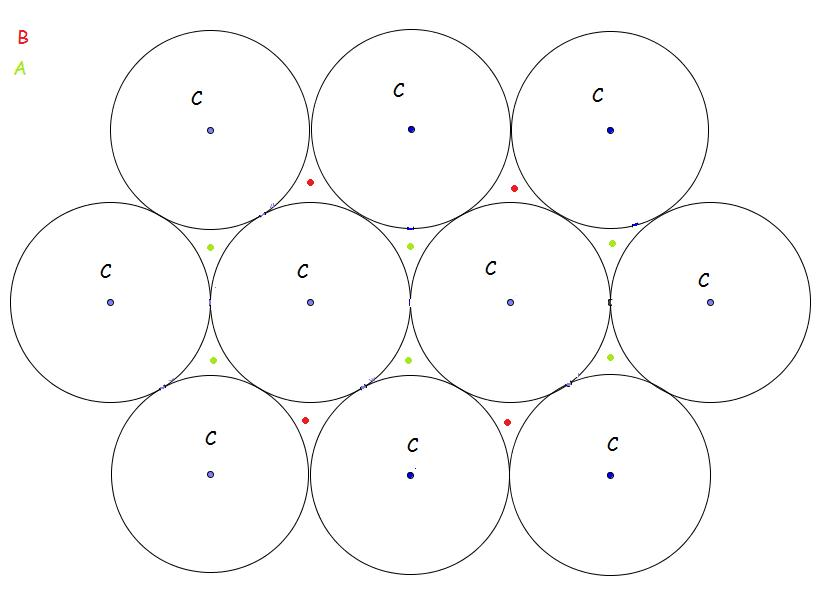
\includegraphics[width=0.5\textwidth]{apunteslattice}
\caption{sphere packing}
\end{figure}

For the next layer we have two options, put them (the centers of the sphere) over the deep holes A or over the deep holes B. For the second layer we put, we will have the possibility of putting them over C (the centers of the spheres of the first layer).
Each lattice obtained by snugly packing copies of $A_2$ is determied by the sequences
ABAB.... (this is the hexagonal close packing(He attoms))
ABCABC....(this is the face-centered cubic lattice ($A_3$))
of equivalence classes of deep holes.

In each step there are two options to choose from, which makes uncountably many possibilities in total.



% Local Variables: 
% mode: latex
% TeX-master: "dag-upc"
% End: 

\scribe{Ane Santos}



\begin{definition}
Informally, an \emph{orbifold} is the quotient of a manifold (here, the Euclidean plane) by the action of a group.
\end{definition}

\begin{displaymath}
	\begin{array}{lcc}
		torus & \longrightarrow & \circ \\
		holes & \longrightarrow & * \\
		non-orientability & \longrightarrow & \times \\
		boundary singularity & \longrightarrow & *n \\
		core point of order n & \longrightarrow & n \
	\end{array}
\end{displaymath}

\begin{theorem}{Magic theorem for the sphere}
The total cost of the signature of any spherical group is $ \$ 2-frac{2}{g} $ where $g=total number of symmetries$
\end{theorem}

The Magic theorem in the plane is a special case because the number of symmetries in a plane is infinite, so the cost is always 2.

There are 14 spherical symmetry groups: $m,n\geq1$

\begin{displaymath}
	\begin{array}{lcccc}
		*532 & *432 & *332 & *22n & *mn \\
		 & & 3*2 & 2*n & n* \\
		 & & & & n\times \\
		 532 & 432 & 332 & 22n & mn 
	\end{array}
\end{displaymath}

If $n\rightarrow\infty$ and $m\rightarrow\infty$ in $*22n$, $*mn$, $2*n$, $n*$, $n\times$, $22n$ and $mn$ we get the 7 possible groups of friezes (cenefas).


\bibliographystyle{amsalpha}
\bibliography{dag}

\end{document}

%%% Local Variables: 
%%% mode: latex
%%% TeX-master: t
%%% End: 
